\documentclass[11pt,a4paper]{article}
\usepackage[top=1.00in, bottom=1.0in, left=1.1in, right=1.1in]{geometry}
\usepackage{graphicx}
\usepackage[numbers]{natbib}
\bibliographystyle{..//..//references/styles/nature.bst}

\usepackage[export]{adjustbox}

\usepackage{Sweave}
\begin{document}

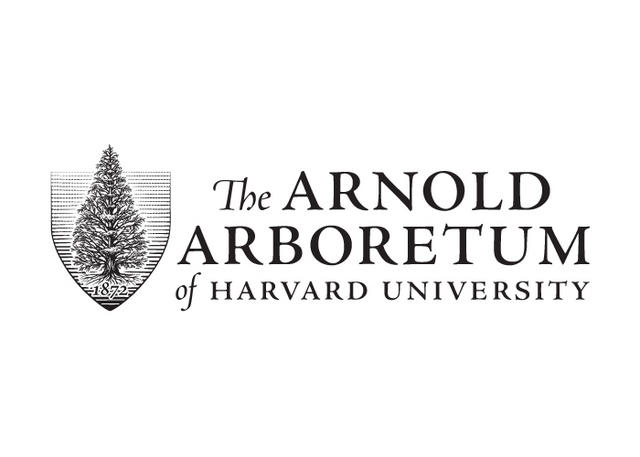
\includegraphics[width=0.5\textwidth, right]{AA_logo.jpg}
\noindent 1300 Centre Street\\
\noindent Boston, MA, 20131\\

\vspace{1.5ex}

\pagenumbering{gobble}

\noindent{Dear Dr. Gibson:}
\vspace{3ex}\\
\noindent Please consider our manuscript, `False spring damage to temperate tree saplings is amplified with winter warming', as a Research Article for the \textit{Journal of Ecology}. \\

\noindent Biological spring is advancing with climate change but late spring freeze dates are not predicted to advance at the same rate, leading to renewed interest in late spring freeze events---commonly called `false springs'---which shape the life history of many temperate and boreal plant species. At the same time over-winter chilling may decrease with warming winters, which could impact plant phenology and, ultimately, growth. Together, false springs and warmer winters could reshape forest plant communities, with cascading effects on pollinators, nutrient cycling and carbon uptake.  \\ % Let's say why this is important early!

\noindent Here, we present an experiment on the interplay of false springs and warmer winters (generally expected to reduce chilling) across eight temperate deciduous tree species examining a suite of phenological, growth and leaf tissue traits. We found that false springs increased tissue damage, decreased leaf toughness, leaf thickness and chlorophyll content, and slowed budburst to leafout timing---extending the period of maximum freezing risk. Chilling, however, shortened this period of maximum risk, even under false spring conditions, thus compensating for some of the more adverse phenological effects of false springs. Despite major shifts in phenology from false springs and chilling we did not find evidence of phenological reordering within the community of species we studied. Our results instead suggest climate change will reshape forest communities through impacts on growth and leaf traits from the coupled effects of false springs and warmer winters under future climate change.\\

\noindent We believe our research is important and timely because our findings contribute to fundamental knowledge on how chilling and freeze events shape tree growth across species, and suggest climate change could diminish or reverse the positive effects of carbon storage in temperate forests. Further, our focus on interactive effects of warmer winters and springs applies widely to a diversity of plant and animal taxa. \\ % I thought it might be nice to connect results beyond plants for the editor.

\noindent This manuscript is not under consideration elsewhere. Both authors approved of this version for submission. We hope that you will find it suitable for publication in the \textit{Journal of Ecology}. Thank you for your consideration. \\

\vspace{1.5ex}
\noindent Sincerely, \\
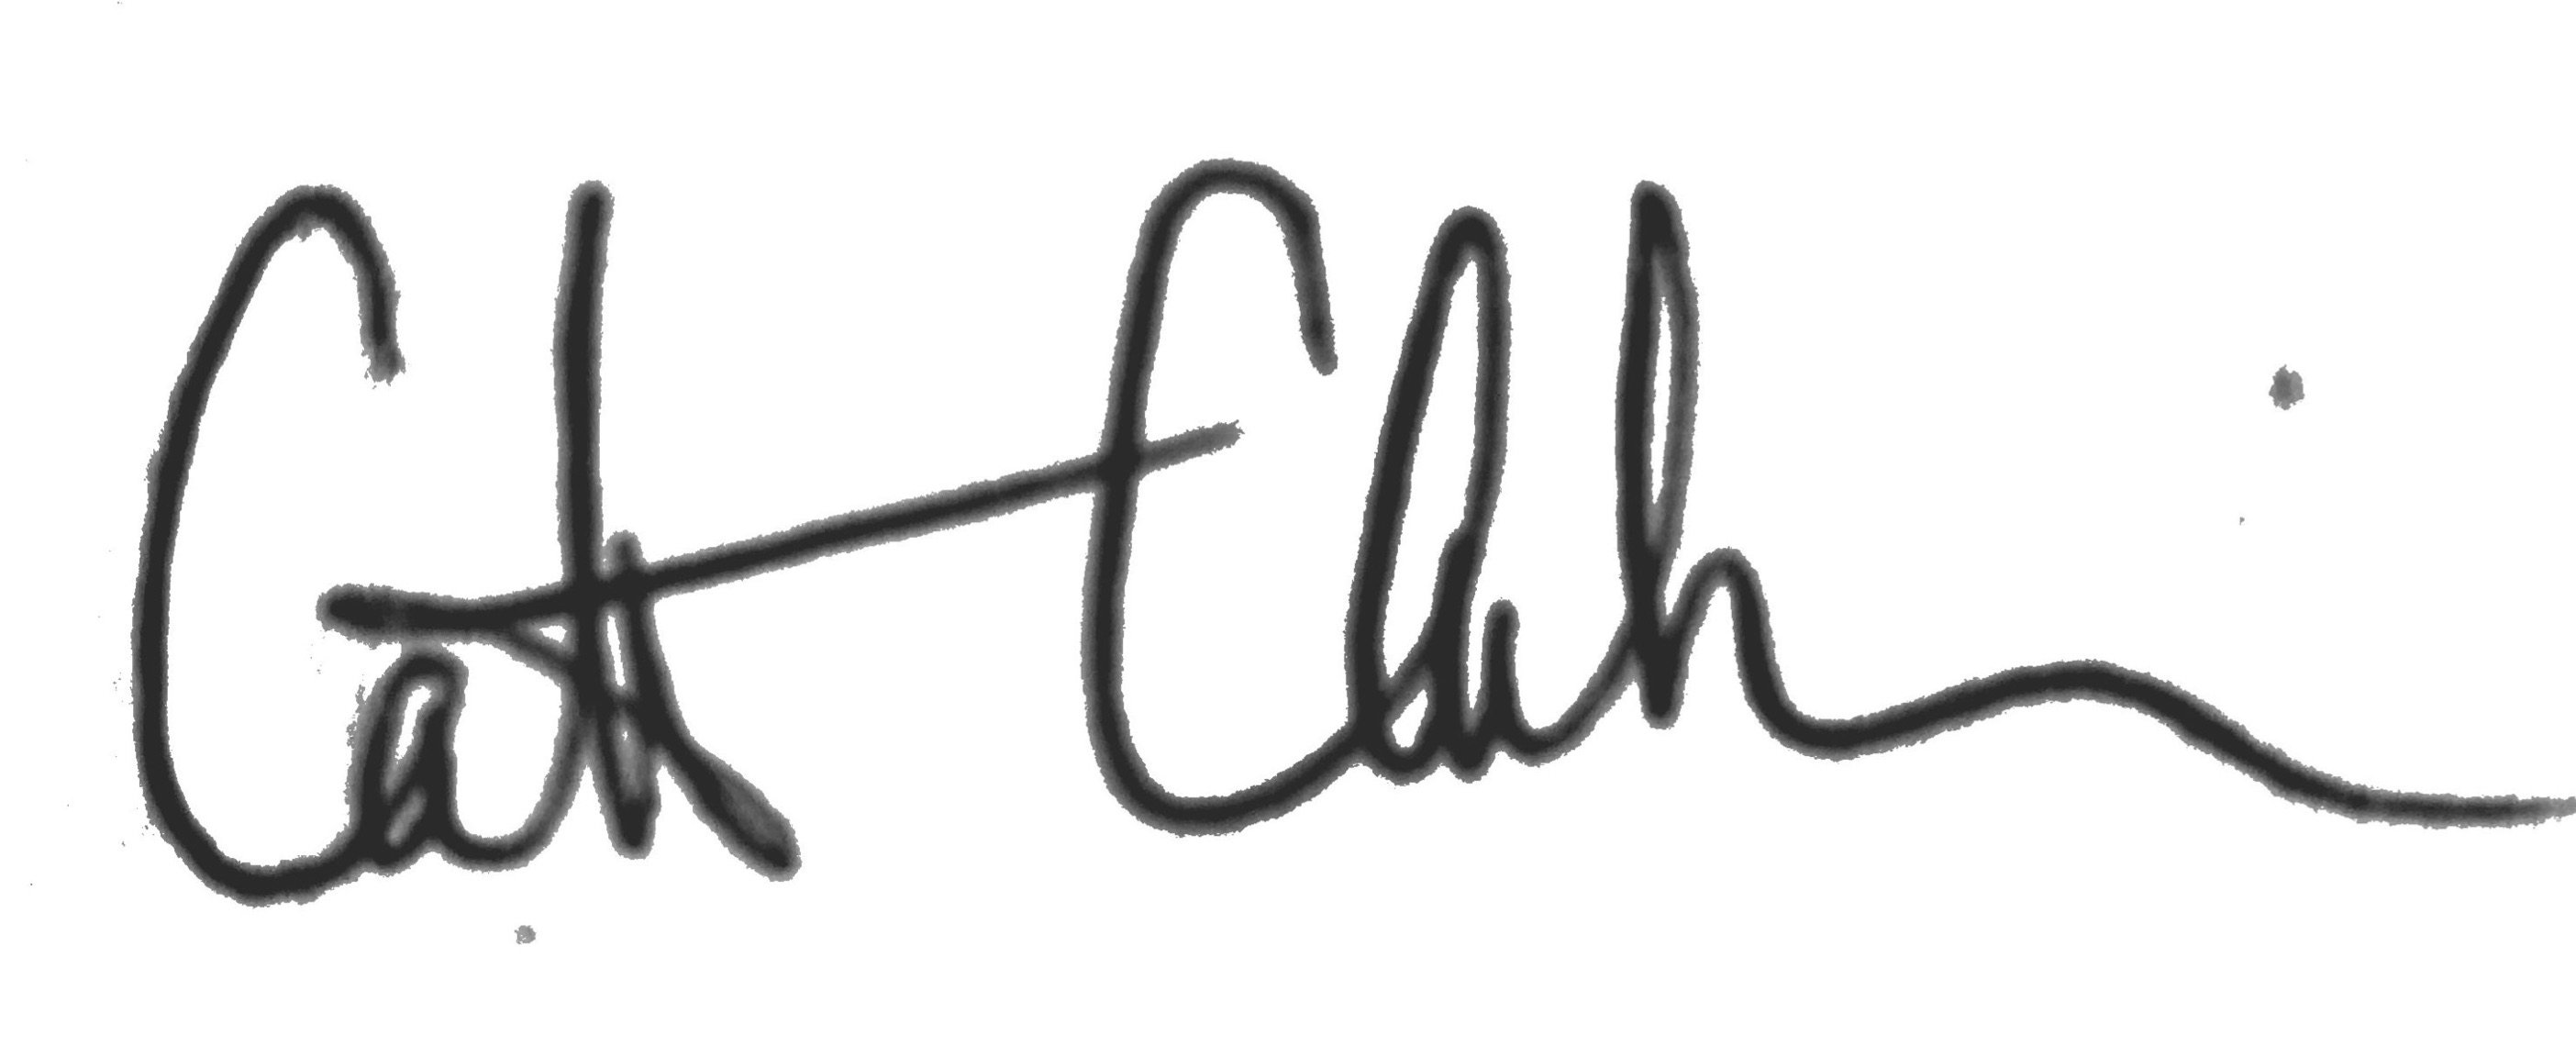
\includegraphics[width=0.2\textwidth]{full_signature.jpg} \\
\noindent Catherine Chamberlain (on behalf of my co-authors)
\vspace{2ex}\\
\noindent Authors:\\
C. J. Chamberlain $^{1,2}$ \& E. M. Wolkovich $^{1,2,3}$
\vspace{2ex}\\
\emph{Author affiliations:}\\
$^{1}$Arnold Arboretum of Harvard University, 1300 Centre Street, Boston, Massachusetts, USA; \\
$^{2}$Organismic \& Evolutionary Biology, Harvard University, 26 Oxford Street, Cambridge, Massachusetts, USA; \\
$^{3}$Forest \& Conservation Sciences, Faculty of Forestry, University of British Columbia, 2424 Main Mall, Vancouver, BC V6T 1Z4\\
\vspace{2ex}
$^*$Corresponding author: 248.953.0189; cchamberlain@g.harvard.edu\\

\bibliography{..//..//references/chillfreeze.bib}

\end{document}
